% FFI26 — SmolVLA trên LIBERO: Reproduce, Analyse, Improve (RL). Bản rút gọn của main.tex (02/11/2026):
% giữ ý chính, bớt số liệu và đường dẫn. Nguồn của từng số: main.tex và report/MAIN_TEX_NOTES.md.
% Biên dịch: cd report && latexmk -xelatex main_revised.tex
\documentclass[10pt,a4paper]{article}

\usepackage{fontspec}
\usepackage{polyglossia}
\setmainlanguage{vietnamese}
\setmainfont{Latin Modern Roman}
\setsansfont{Latin Modern Sans}
\setmonofont{Latin Modern Mono}

\usepackage[margin=2.1cm,top=2cm,bottom=2.2cm]{geometry}
\usepackage{amsmath,amssymb,mathtools}
\usepackage{graphicx}
\usepackage{booktabs,tabularx,multirow,makecell}
\usepackage{enumitem}
\usepackage{xcolor}
\usepackage{caption,subcaption}
\usepackage{float}
\usepackage[hidelinks]{hyperref}
\usepackage{tikz}
\usetikzlibrary{arrows.meta,positioning,fit,backgrounds,calc,shapes.geometric}

\graphicspath{{figures/}}
\setlist{itemsep=1pt,topsep=3pt,leftmargin=1.3em}
\captionsetup{font=small,labelfont=bf,skip=4pt}
\setlength{\parskip}{2pt}

\definecolor{cV4}{HTML}{E6550D}
\definecolor{cS}{HTML}{EFF3FF}\definecolor{cR}{HTML}{FEE6CE}\definecolor{cA}{HTML}{E5F5E0}\definecolor{cI}{HTML}{FCBBA1}
\newcommand{\code}[1]{\texttt{\detokenize{#1}}}
\newcommand{\Lhat}{\hat{\mathcal{L}}}
\newcommand{\thold}{\theta_{\text{old}}}
\newcommand{\up}{\textcolor{green!50!black}{$\blacktriangle$}}
\newcommand{\dn}{\textcolor{red!70!black}{$\blacktriangledown$}}
\newcommand{\review}[1]{\fcolorbox{orange}{orange!8}{\parbox{0.97\linewidth}{\scriptsize\textcolor{orange!70!black}{\textbf{[Cần bạn điền / kiểm tra]} #1}\\[1.6em]}}}
\newcommand{\reviewinline}[1]{\fcolorbox{orange}{orange!8}{\scriptsize\textcolor{orange!70!black}{#1}\hspace{3em}}}
\newcommand{\figorbox}[2]{\IfFileExists{figures/#1}{\includegraphics[width=#2]{#1}}{\fbox{\parbox[c][2.5cm][c]{#2}{\centering\small thiếu \code{figures/#1}}}}}

\title{\textbf{Fine-tune SmolVLA trên LIBERO-Long bằng học tăng cường}\\[2pt]
\large Study $\cdot$ Reproduce $\cdot$ Analyse $\cdot$ Improve}
\author{Nguyễn Thị Ngọc Lan, email: nguyenngoclanuet@gmail.com}
\date{2/11/2026}

\begin{document}
\maketitle
\vspace{-1.2em}

\section*{Tóm tắt}
\begin{itemize}
\item \textbf{Reproduce.} Checkpoint công bố \code{lerobot/smolvla_libero} đạt 72{,}8\% trên LIBERO-10 khi thực thi 10 hành
động rồi mới quan sát lại (NAS=10). Với NAS=1 và NAS=50, kết quả chỉ còn 54{,}6\% và 47{,}8\%.
\item \textbf{Analyse.} SmolVLA hiểu đúng câu lệnh và làm tốt task một bước. Nó yếu ở task hai vật: thường xong vật thứ
nhất rồi dừng, và hay gắp hỏng.
\item \textbf{Improve.} Fine-tune action expert bằng FPO (RL on-policy) trên task 0 và task 8. Bản cuối (FPO v4) tăng tỉ lệ
thành công trên hai task này từ 40{,}3\% lên 46{,}7\% ($p=0{,}025$), không làm giảm 8 task còn lại. Mức tăng đến từ việc
policy chuyển được sang vật thứ hai; lỗi gắp chưa được sửa.
\end{itemize}

% ===================================================================== overview diagram
\begin{figure}[H]
\centering
\begin{tikzpicture}[font=\scriptsize, >=Stealth,
  ph/.style={draw, rounded corners=3pt, minimum height=1.0cm, text width=3.1cm, align=center, inner sep=3pt},
  ar/.style={->, thick}]
\node[ph, fill=cS] (S) at (0,0) {\textbf{1. Study}\\đọc tài liệu RL cho VLA};
\node[ph, fill=cR] (R) at (4.3,0) {\textbf{2. Reproduce}\\chọn NAS = 10};
\node[ph, fill=cA] (A) at (8.6,0) {\textbf{3. Analyse}\\chọn task 0, 8};
\node[ph, fill=cI] (I) at (12.9,0) {\textbf{4. Improve}\\FPO v1 $\to$ v4};
\draw[ar] (S) -- (R); \draw[ar] (R) -- (A); \draw[ar] (A) -- (I);
\end{tikzpicture}
\caption{Luồng công việc.}
\label{fig:flow}
\end{figure}

% ===================================================================== REPRODUCE
\section{Reproduce}

\begin{figure}[H]
\centering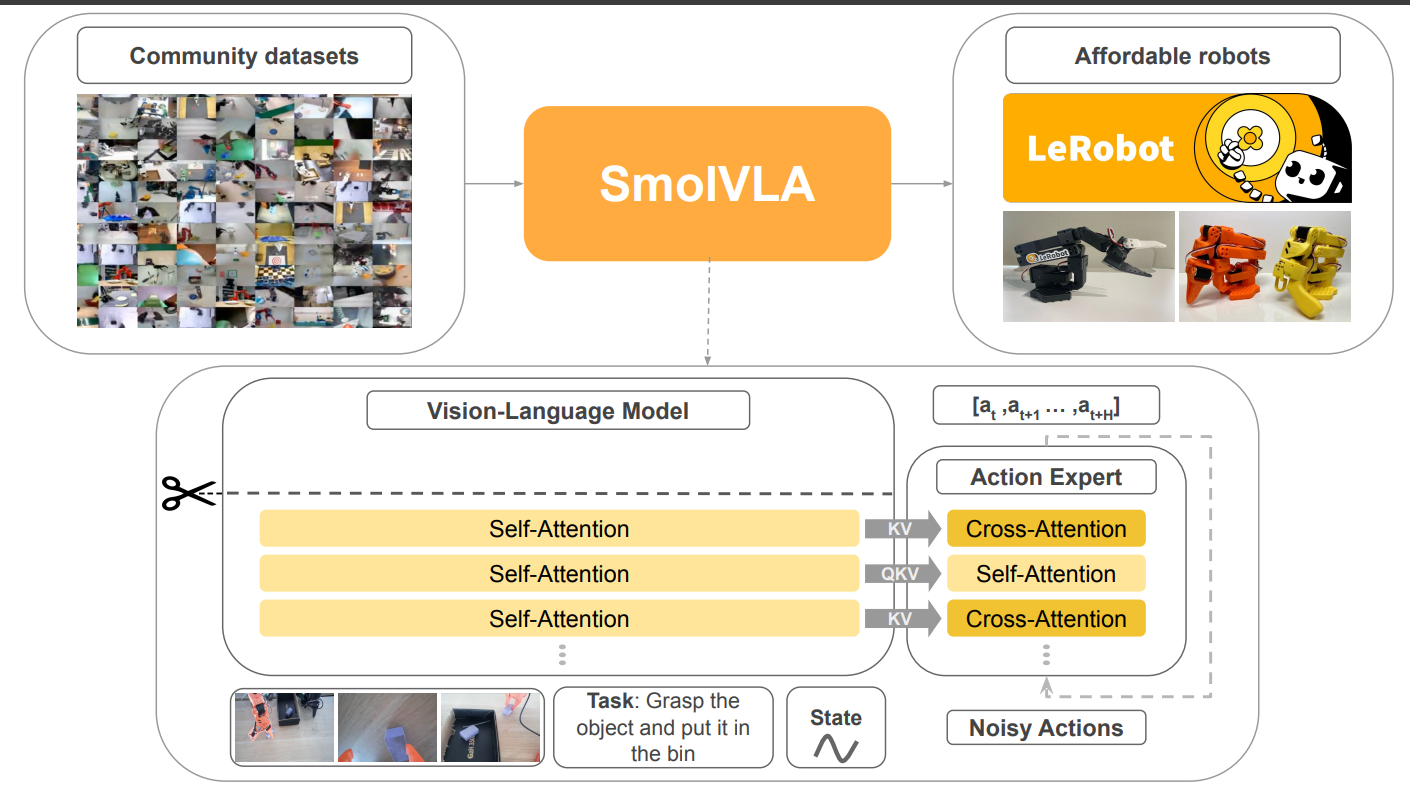
\includegraphics[width=0.8\linewidth]{overview_smolvla.png}
\caption{Kiến trúc SmolVLA.}
\label{fig:arch}
\end{figure}

\paragraph{SmolVLA sinh hành động như thế nào?}
Hai ảnh camera, câu lệnh và trạng thái robot đi qua VLM SmolVLM2. Action expert đọc đặc trưng của VLM, rồi biến một nhiễu
ngẫu nhiên thành một chunk 50 hành động qua 10 bước khử nhiễu. Robot thực thi NAS hành động đầu của chunk, rồi quan sát
lại và sinh chunk mới.

\paragraph{Thiết lập.} Dùng đúng checkpoint của tác giả, không train lại. Mỗi episode tối đa 520 bước; thành công khi mọi
điều kiện đích của task đều đúng.

\begin{table}[H]
\centering\footnotesize
\begin{tabular}{@{}l c c c@{}}
\toprule
Suite & NAS=1 & \textbf{NAS=10} & NAS=50 \\
\midrule
LIBERO-10 (Long) & 54{,}6\% & \textbf{72{,}8\%} & 47{,}8\% \\
LIBERO-Spatial & 79{,}0\% & 82\% & 58\% \\
\bottomrule
\end{tabular}
\caption{Tỉ lệ thành công của \code{lerobot/smolvla_libero} theo NAS. Bài SmolVLA báo 71\% (Long) và 90\% (Spatial).}
\label{tab:repro}
\end{table}

\noindent Cùng một checkpoint, chỉ đổi NAS đã làm kết quả chênh tới 25 điểm. NAS=10 tốt nhất nên được giữ cho mọi
phần sau. Như vậy mọi cải thiện ở phần Improve là nhờ RL, không phải nhờ đổi cách thực thi.

% ===================================================================== ANALYSE
\section{Analyse}\label{sec:analyse}

\paragraph{Dữ liệu.} Toàn bộ phần này dùng một bộ dữ liệu: SmolVLA gốc với NAS=10, mỗi task 50 cảnh $\times$ 3 seed
(150 episode/task, 1500 episode). Đây cũng chính là bản gốc được so sánh ở phần Improve. Mỗi episode lưu vị trí các vật
và trạng thái của từng điều kiện đích ở mọi bước, nên ngoài thành công/thất bại còn biết được robot hỏng ở đâu. Tỉ lệ
chung là 69{,}1\%, thấp hơn 72{,}8\% ở Reproduce một chút vì khác seed và khác script eval.

\begin{table}[H]
\centering\small
\begin{tabular}{@{}c l r@{}}
\toprule
Task & Việc cần làm & Thành công \\
\midrule
3 & bát vào ngăn kéo dưới, rồi đóng ngăn kéo & 97\% \\
2 & bật bếp, rồi đặt ấm moka lên & 91\% \\
5 & sách vào ngăn sau của giá & 89\% \\
1 & hộp cream cheese và bơ vào giỏ & 83\% \\
9 & cốc vào lò vi sóng, rồi đóng lò & 75\% \\
7 & lon alphabet soup và hộp cream cheese vào giỏ & 69\% \\
4 & hai cốc lên hai đĩa trái/phải & 54\% \\
6 & cốc lên đĩa, hộp pudding sang phải đĩa & 52\% \\
\textbf{0} & lon alphabet soup và lon tomato sauce vào giỏ & \textbf{41\%} \\
\textbf{8} & hai ấm moka lên bếp & \textbf{40\%} \\
\bottomrule
\end{tabular}
\caption{Tỉ lệ thành công của SmolVLA gốc theo task (150 episode/task), xếp từ cao xuống thấp.}
\label{tab:tasks}
\end{table}

\begin{table}[H]
\centering\small
\begin{tabularx}{\linewidth}{@{}p{0.36\linewidth} X@{}}
\toprule
\textbf{Điểm mạnh} & \textbf{Bằng chứng} \\
\midrule
S1: task một vật, hoặc một vật + một thao tác khớp nối & task 3, 2, 5 đều trên 88\% (Bảng~\ref{tab:tasks}) \\
S2: hiểu đúng câu lệnh & chỉ 11/464 thất bại có cầm vật không thuộc câu lệnh, cả 11 ở task 0 \\
S3: thực thi theo chunk rồi quan sát lại nên sửa được sai & 84 episode thành công có lúc vật trượt khỏi kẹp, rồi gắp lại được \\
S4: nhỏ, nhanh & 450M tham số; train, eval, RL đều chạy trên 1 GPU 16\,GB \\
\midrule
\textbf{Giới hạn} & \\
\midrule
L1: xong vật thứ nhất rồi không xong vật thứ hai & 253/464 thất bại kết thúc khi đã xong một phần; task 8: 75/90 \\
L2: thao tác chưa khéo (7 loại, Bảng~\ref{tab:l2}) & 310/464 thất bại có ít nhất một lỗi thao tác, so với 28/1036 episode thành công \\
L3: nhạy với cách thực thi & đổi NAS làm chênh 25 điểm (Bảng~\ref{tab:repro}) \\
\bottomrule
\end{tabularx}
\caption{Điểm mạnh và giới hạn của SmolVLA gốc trên LIBERO-10.}
\label{tab:analyse}
\end{table}

\paragraph{L2 chi tiết: SmolVLA hỏng ở những thao tác nào?} Các lỗi được nhận ra tự động từ vị trí vật và trạng thái kẹp
ở từng bước. Một episode có thể mắc nhiều lỗi. Riêng lỗi kẹp sai tư thế thì không nhận ra được tự động, vì log không có
hướng của vật.

\begin{table}[H]
\centering\small
\begin{tabularx}{\linewidth}{@{}p{0.2\linewidth} X c p{0.25\linewidth}@{}}
\toprule
Lỗi & Cách nhận biết & \makecell{Thất bại /\\thành công} & Gặp nhiều ở \\
\midrule
L2a gắp hỏng & đóng kẹp nhiều lần sát vật cần lấy, nhưng không nhấc được vật & \textbf{193} / 0 & task 0, 6, 7, 8 \\
L2b trượt khỏi kẹp & vật tuột ra khi kẹp vẫn đóng & 203 / 84 & task 0, 6, 7 \\
L2c chạm vật khác & chạm làm xô lệch, hoặc cầm, vật không thuộc câu lệnh & 46 / 8 & task 0, 1 \\
L2d làm rơi & vật đang mang rơi xuống & 51 / 7 & task 7, 1, 9 \\
L2e kẹp sai tư thế & không đo được tự động & --- & ví dụ ở Hình~\ref{fig:fail}b \\
L2f đặt lệch & vật đã được đặt xuống sát đích nhưng chưa đủ gần để tính là đúng & 76 / 12 & task 4, 6 \\
L2g làm mất tiến độ & vật đã đúng chỗ lại bị kéo ra & 25 / 4 & rải rác \\
\bottomrule
\end{tabularx}
\caption{Các lỗi thao tác của SmolVLA gốc. Cột giữa: số episode mắc lỗi, trên 464 thất bại và 1036 thành công.}
\label{tab:l2}
\end{table}

\noindent Ba điểm rút ra:
\begin{enumerate}
\item \textbf{Gắp hỏng là lỗi thao tác chính.} Nó có ở 193/464 thất bại và không có ở episode thành công nào. Lỗi nặng
nhất ở task 0: robot với vào cụm hộp nơi lon alphabet soup nằm khuất, hay chạm phải hộp nước cam, và 68/89 thất bại kết
thúc khi chưa đưa được lon nào vào giỏ.
\item \textbf{Hai nhóm task hỏng theo hai cách khác nhau.} Ở task 0 và 7, robot thường hỏng ngay từ lúc gắp vật đầu tiên
(L2). Ở task 8 và 4, robot thường đã xong vật thứ nhất nhưng không xong vật thứ hai (L1): 75/90 và 57/69 thất bại.
\item \textbf{Đặt chưa đủ chính xác} (L2f) tập trung ở các task đặt cốc lên đĩa (task 4, 6): vật nằm sát đĩa nhưng lệch
ra ngoài.
\end{enumerate}

\begin{figure}[H]
\centering
\begin{subfigure}{\linewidth}\centering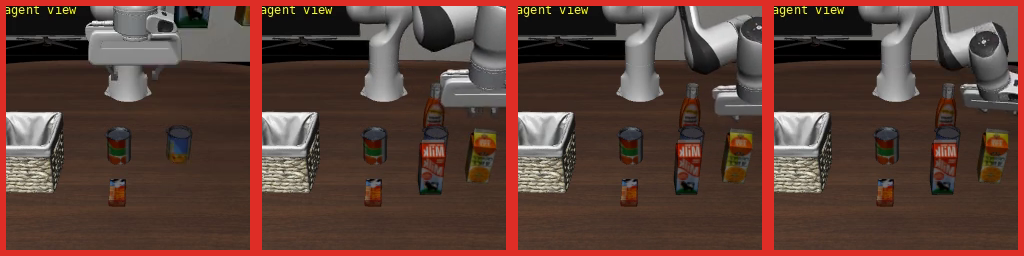
\includegraphics[width=\linewidth]{fail_base_t0_init2_s5000.png}
\caption{Task 0 (L2a): robot loay hoay ở cụm hộp phía sau, đóng kẹp nhiều lần nhưng không nhấc được lon nào tới hết giờ.}
\end{subfigure}\\[3pt]
\begin{subfigure}{\linewidth}\centering
\includegraphics[width=\linewidth]{fail_base_t8_init2_s3000.png}
\caption{Task 8 (L1, L2e): ấm thứ nhất đã lên bếp; ấm thứ hai bị kẹp nằm ngang và giữ như vậy tới hết giờ.}
\end{subfigure}
\caption{Hai thất bại điển hình của SmolVLA gốc, lấy từ bộ dữ liệu trên. Mỗi dải: 4 khung đều nhau từ đầu tới cuối episode.}
\label{fig:fail}
\end{figure}

\paragraph{Hệ quả cho Improve.} L3 đã được xử lý bằng NAS=10. L1 và L2 nằm trong chính policy, nên đó là việc của RL.
Improve tập trung vào hai task yếu nhất: \textbf{task 0} (hai lon vào giỏ, lỗi chủ yếu là L2) và \textbf{task 8} (hai ấm
lên bếp, lỗi chủ yếu là L1). Cả hai thành công khoảng 40\%, tức policy đôi khi đã làm được, nên RL có rollout tốt
để học theo.

% ===================================================================== IMPROVE
\section{Improve: RL cho SmolVLA}

\subsection{Hypothesis}\label{sec:hyp}

\paragraph{Vì sao RL có thể sửa được mà BC không sửa được?}
BC chỉ học từ demo thành công. Trên horizon dài, lệch nhỏ ở đầu tích lũy thành thất bại ở cuối, và những trạng thái như
lúc vừa đặt xong ấm thứ nhất, hay lúc lon vừa trượt khỏi kẹp, hiếm khi có trong demo. RL học trên chính các trạng thái mà
policy gặp, và đẩy policy về phía cách xử lý dẫn tới bước tiếp theo.

\paragraph{Giả thuyết.} Fine-tune action expert bằng FPO, với reward thưởng theo tiến độ và phạt lỗi thao tác, sẽ:
\begin{enumerate}[label=\textbf{H\arabic*}]
\item tăng tỉ lệ thành công trên task 0 + 8;
\item nhờ giảm lỗi L1 (xong một vật rồi dừng);
\item giảm lỗi L2 (trượt, chạm vật khác, làm rơi);
\item không làm giảm 8 task còn lại.
\end{enumerate}

% ---------------------------------------------------------------------
\subsection{RL Algorithm: FPO}\label{sec:algo}

\paragraph{Vấn đề.} Theo \code{modeling_smolvla.py}, gọi $a$ là chunk hành động, $\varepsilon\sim\mathcal N(0,I)$ là
nhiễu, $\tau\in[0,1]$ là thời điểm ($\tau=1$ là nhiễu thuần):
\begin{equation}
x_\tau=\tau\varepsilon+(1-\tau)a,\qquad
\mathcal L_\theta(a;o)=\mathbb E_{\tau,\varepsilon}\big\|v_\theta(x_\tau,\tau,o)-(\varepsilon-a)\big\|^2 .
\end{equation}
Policy chỉ ngẫu nhiên nhờ nhiễu ban đầu; quá trình khử nhiễu là tất định. Vì vậy $\log\pi_\theta(a\mid o)$ không tính được,
trong khi PPO cần nó.

\paragraph{Ý tưởng của FPO.} Thay tỉ lệ $\pi_\theta/\pi_{\text{old}}$ của PPO bằng exp của chênh lệch loss flow matching
trên chính chunk đã thực thi (McAllister và cộng sự, 2025):
\begin{equation}
\hat r(\theta)=\exp\!\big(c\,[\Lhat_{\thold}(a;o)-\Lhat_\theta(a;o)]\big),\qquad
J(\theta)=\mathbb E\big[\min\big(\hat r\hat A,\ \operatorname{clip}(\hat r,1\pm\epsilon)\hat A\big)\big].
\end{equation}
Nghĩa là: chunk có advantage dương thì loss của nó được kéo nhỏ lại, tức dễ được sinh ra hơn; chunk có advantage âm thì
ngược lại. Bộ sinh hành động giữ nguyên, chỉ thay loss.

\paragraph{Vì sao chọn FPO?} SmolVLA có cùng kiểu kiến trúc với $\pi_0$, và FPO đã cải thiện được $\pi_0$ trên LIBERO
(Lyu và cộng sự, 2025). Ở bài đó $\pi_0$ được giữ nguyên, FPO chỉ train một mạng nhỏ sinh đầu vào cho $\pi_0$; báo cáo này
thì áp dụng FPO trực tiếp lên action expert của SmolVLA, như bài FPO gốc. FPO cũng rẻ: vừa một GPU 16\,GB. Ở vòng sàng lọc, nó là phương pháp duy nhất tốt hơn checkpoint gốc
(Mục~\ref{sec:screen}).

\paragraph{Advantage tính thế nào?} Không dùng critic. Mỗi cảnh được chạy 8 lần. Mỗi episode được chia thành các đoạn,
ranh giới là lúc một vật đích vừa vào đúng chỗ. Một đoạn có advantage dương nếu nó tới mốc kế tiếp tốt hơn trung bình 8
lần chạy cùng cảnh.

% ---------------------------------------------------------------------
\subsection{Reward}\label{sec:reward}
\begin{equation}
r_t=\underbrace{1[\text{thành công}]}_{\text{mục tiêu}}
+\underbrace{0{,}5\,\big(\gamma\Phi(s_{t+1})-\Phi(s_t)\big)}_{\text{tiến độ}}
-\underbrace{\text{phạt lỗi}}_{\text{slip, va chạm, làm rơi, hết giờ}},
\qquad \Phi(s)=\text{tỉ lệ vật đích đã đúng chỗ}.
\end{equation}
Thành phần tiến độ thưởng ngay khi một vật vào đúng chỗ (nhắm vào L1); các khoản phạt 0{,}1--0{,}2 nhắm vào L2. Dạng
shaping này không đổi policy tối ưu (Ng và cộng sự, 1999).

% ---------------------------------------------------------------------
\subsection{Môi trường và thành phần được train}\label{sec:env}
\begin{itemize}
\item \textbf{Môi trường:} LIBERO-10, cùng thiết lập như Reproduce (NAS=10). Train trên task 0 và 8, mỗi task 16 cảnh;
34 cảnh còn lại mỗi task để kiểm tra (held-out). Mỗi vòng thu 256 episode, tổng 4 vòng.
\item \textbf{Được train:} chỉ action expert (khoảng 100M trên 450M tham số). VLM đóng băng.
\item \textbf{Vì sao?} L1 và L2 là lỗi hành động, không phải lỗi hiểu câu lệnh, và action expert là phần sinh ra
hành động. Giữ nguyên VLM cũng giảm rủi ro quên các task khác.
\end{itemize}

% ---------------------------------------------------------------------
\subsection{Vòng sàng lọc}\label{sec:screen}
Trước khi đi sâu vào FPO, ba hướng được thử nhanh trên cùng một phép đo: task 0 và 8, mỗi task 50 cảnh, một seed
(100 episode), so theo cặp với SmolVLA gốc. Trên phép đo này SmolVLA gốc đạt 44\%.
\begin{itemize}
\item \textbf{A1, gắn nhãn advantage (kiểu RECAP).} Khi train, mỗi mẫu được gắn nhãn tốt hoặc xấu theo advantage,
vào câu lệnh hoặc qua một embedding học được; khi chạy thì gắn nhãn tốt. Kết quả 31--44\%, không bản nào hơn
bản gốc; gắn nhãn tốt vào câu lệnh còn kém hơn (31\%, $p=0{,}04$). Nhãn tốt và xấu cho kết quả gần như nhau,
tức mô hình không học được ý nghĩa của nhãn.
\item \textbf{A2, AWR.} Loss flow matching được nhân trọng số theo advantage. Kết quả 41--47\%, không khác bản gốc, kể
cả khi train tới 6000 bước.
\item \textbf{FPO.} Sau vòng 2 và vòng 3 đạt 56\% và 57\%, tốt hơn bản gốc có ý nghĩa ($p=0{,}01$). Đây là hướng duy nhất
có tác dụng, nên được chọn để phát triển tiếp.
\end{itemize}
\paragraph{Vì sao A1 và A2 không có tác dụng?} Lúc đó action expert được nạp ở bf16. Mỗi bước cập nhật nhỏ hơn độ phân
giải của bf16 nên bị làm tròn mất: sau 6000 bước chỉ 5{,}5\% phần tử của expert thay đổi. Phát hiện này dẫn tới FPO v2
(giữ trọng số ở fp32). Ngoài ra, khi đo lại bằng phép đo cuối (expert fp32, 3 seed), FPO v1 không giữ được mức 57\%
(Bảng~\ref{tab:final}); vì vậy mọi so sánh sau đây đều dùng phép đo cuối.

\subsection{Chuỗi phiên bản FPO}
\begin{table}[H]
\centering\small
\begin{tabularx}{\linewidth}{@{}l X X@{}}
\toprule
Bản & Thay đổi & Vì sao \\
\midrule
v1 & FPO cơ bản & --- \\
v2 & trọng số fp32, batch lớn hơn, neo về rollout thành công & v1: cập nhật bị làm tròn ở bf16, tín hiệu nhiễu \\
v3 & thêm demo của cả 10 task khi train & v2: quên 8 task còn lại \\
v4 & sửa cách cân advantage theo đoạn & v3: rollout thất bại dài hơn nên bị cân lệch, task 0 giảm \\
\bottomrule
\end{tabularx}
\caption{Mỗi bản chỉ đổi một nhóm thay đổi; mọi thứ khác giữ nguyên.}
\label{tab:versions}
\end{table}

% ---------------------------------------------------------------------
\subsection{Kết quả}
Mỗi model được chạy trên cùng các cảnh và seed, rồi so theo cặp với SmolVLA gốc (kiểm định McNemar).

\begin{table}[H]
\centering\small
\setlength{\tabcolsep}{5pt}
\begin{tabular}{@{}l c c c c c@{}}
\toprule
& gốc & FPO v1 & FPO v2 & FPO v3 & \textbf{FPO v4} \\
\midrule
task 0 & 41\% & 41\% & 33\% & 31\% \dn & \textbf{40\%} \\
task 8 & 40\% & 24\% \dn & 51\% & 59\% \up & \textbf{53\%} \up \\
task 0 + 8 & 40{,}3\% & 32{,}7\% \dn & 42{,}0\% & 44{,}7\% & \textbf{46{,}7\%} \up \\
8 task còn lại & 79\% & 69\% \dn & 68\% \dn & 72\% \dn & \textbf{78\%} \\
\bottomrule
\end{tabular}
\caption{Tỉ lệ thành công. \up/\dn: tốt hơn/kém hơn bản gốc có ý nghĩa ($p<0{,}05$).}
\label{tab:final}
\end{table}

\begin{figure}[H]
\centering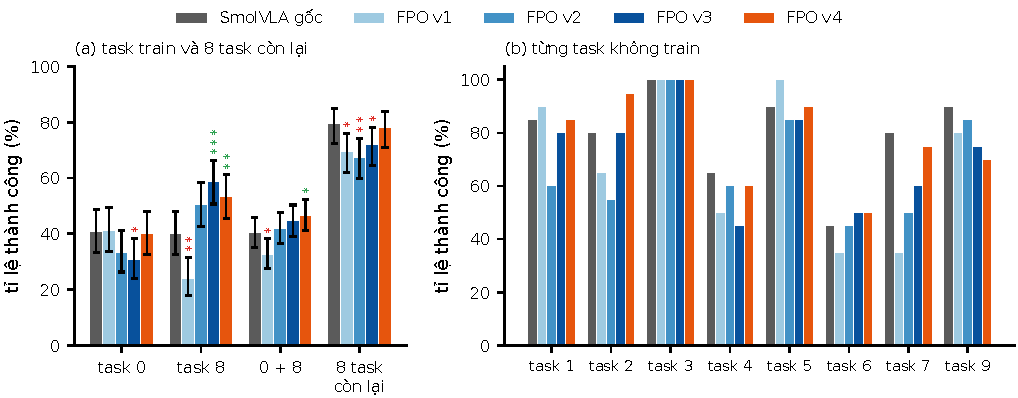
\includegraphics[width=\linewidth]{fig_fpo_final_simple.pdf}
\caption{So sánh cuối giữa SmolVLA gốc và các phiên bản FPO. Thanh lỗi: khoảng tin cậy 95\%. Dấu sao: khác bản gốc có ý nghĩa (xanh: tốt hơn, đỏ: kém hơn).}
\label{fig:final}
\end{figure}

\subsection{Giả thuyết nào đúng?}\label{sec:verify}
\begin{itemize}
\item \textbf{H1 đúng.} Task 0 + 8 tăng từ 40{,}3\% lên 46{,}7\% ($p=0{,}025$). Toàn bộ mức tăng nằm ở task 8; task 0 giữ
nguyên.
\item \textbf{H2 đúng ở task 8.} Số thất bại mà robot xong một ấm rồi dừng giảm từ 75 xuống 53 ($p=0{,}002$). RL đã dạy policy
chuyển sang ấm thứ hai, đúng điều reward tiến độ thưởng.
\item \textbf{H3 chưa đúng.} Trượt, va chạm, làm rơi và gắp hỏng không giảm có ý nghĩa. Vì vậy task 0, nơi lỗi chủ yếu
là gắp, không tăng.
\item \textbf{H4 đúng.} 8 task còn lại giữ nguyên (78\% so với 79\%, $p=0{,}83$). Các bản trước v4 đều làm giảm.
\end{itemize}

\paragraph{Vì sao L2 chưa sửa được?} Khả năng cao là vì cập nhật quá nhỏ: trọng số chỉ thay đổi dưới 0{,}15\%, vì cơ chế
clip của PPO dừng mỗi vòng rất sớm. Ngoài ra, phạt lỗi (0{,}1--0{,}2) nhỏ so với thưởng thành công (1), và gắp hỏng không
có khoản phạt riêng. Các giải thích này chưa được kiểm chứng.

\subsection{Ví dụ}
\begin{figure}[H]
\centering\figorbox{fig_keyframes.pdf}{\linewidth}
\caption{Cùng một cảnh: SmolVLA gốc, FPO v3, FPO v4. Viền xanh: thành công; đỏ: thất bại.}
\label{fig:keyframes}
\end{figure}
Hình~\ref{fig:keyframes} so sánh SmolVLA gốc, FPO v3 và FPO v4 trên ba cảnh của phép đo cuối (video của các cảnh này có
trong thư mục kết quả thực nghiệm).
\begin{itemize}
\item \textbf{Task 0, init 4, seed 5000.} Cả ba model đều nhấc được lon thứ nhất. Với lon thứ hai, cả ba đều gắp trượt.
SmolVLA gốc và FPO v3 thử lại nhiều lần nhưng vẫn hụt, và thất bại khi hết 520 bước. FPO v4 chỉnh càng kẹp sát về phía lon,
gắp được và thành công ở bước 498.
\item \textbf{Task 8, init 0, seed 3000.} SmolVLA gốc và FPO v3 đều đặt được ấm thứ nhất lên bếp. Với ấm thứ hai, càng kẹp
bám vào đầu ấm rồi đứng yên tới hết giờ (lỗi L1). FPO v4 đặt được cả hai ấm và thành công ở bước 391.
\item \textbf{Task 8, init 6, seed 3000.} Trường hợp ngược lại: SmolVLA gốc và FPO v3 thành công (bước 386 và 379). FPO v4
gắp ấm thứ nhất nhanh nhưng không chắc, làm rơi ấm; sau đó vẫn đặt được ấm thứ hai, nhưng episode thất bại khi hết 520 bước.
\end{itemize}

% ===================================================================== CONCLUSION
\section{Hạn chế và hướng tiếp theo}
\begin{itemize}
\item Mỗi phiên bản chỉ train một lần, nên khác biệt giữa các bản có thể một phần do ngẫu nhiên.
\item Nhãn lỗi là tự động, chưa kiểm hết bằng video.
\item Chỉ train 2/10 task; chưa thử Flow-SDE (tính log-prob chính xác).
\end{itemize}
\paragraph{Hướng tiếp theo: DSRL} (Wagenmaker và cộng sự, 2025). Giữ nguyên SmolVLA, học một policy nhỏ chọn nhiễu ban đầu
$\varepsilon$ của flow matching, nên không cần gradient qua VLA. Đề xuất này xuất phát từ hai quan sát ở kết quả FPO:
\begin{itemize}
\item \textbf{Sửa trọng số dễ gây quên.} v1--v3 đều làm giảm 8 task còn lại; phải thêm demo của cả 10 task và sửa cách
cân advantage (v4) mới giữ được. DSRL không đụng vào trọng số SmolVLA nên tránh được vấn đề này từ đầu.
\item \textbf{Phần FPO sửa được là hành vi SmolVLA đã có sẵn.} Advantage được tính so với 8 lần chạy cùng cảnh, nên FPO
chỉ học được từ những lần SmolVLA đã tự làm tốt hơn (ví dụ chuyển sang ấm thứ hai ở task 8). Chọn nhiễu ban đầu là cách
trực tiếp hơn để luôn lấy ra những hành vi tốt đó.
\end{itemize}
Kỳ vọng (chưa kiểm chứng): giữ được mức tăng ở task 8 mà không gây quên. Đổi lại, DSRL chỉ chọn được trong những hành vi
SmolVLA đã tạo ra được từ nhiễu, nên có thể cũng không sửa được lỗi gắp ở task 0 (H3). Báo cáo này chưa đánh giá DSRL.


\section*{Tài liệu tham khảo}
{\scriptsize\raggedright
\begin{itemize}
\item Shukor và cộng sự (2025). SmolVLA. arXiv:2506.01844.
\item McAllister và cộng sự (2025). Flow Matching Policy Gradients (FPO). arXiv:2507.21053.
\item Lyu và cộng sự (2025). Reinforcement Fine-Tuning of Flow-Matching Policies for VLA Models ($\pi_0$-FPO). arXiv:2510.09976.
\item Ng, Harada, Russell (1999). Policy invariance under reward transformations: theory and application to reward shaping. ICML.
\item Chen và cộng sự (2025). $\pi_{\text{RL}}$: Online RL fine-tuning for flow-based VLA. arXiv:2510.25889.
\item Physical Intelligence (2025). $\pi^*_{0.6}$ / RECAP. arXiv:2511.14759.
\item Wagenmaker và cộng sự (2025). Steering diffusion policy with latent space RL (DSRL). arXiv:2506.15799.
\item Liu và cộng sự (2023). LIBERO. NeurIPS Datasets and Benchmarks.
\end{itemize}}

\end{document}
